\documentclass[a4paper,12pt]{article}
\usepackage[english]{babel}
\usepackage[utf8]{inputenc}
\usepackage{amsmath}
\usepackage{amsthm}
\usepackage{amsfonts}
\usepackage{amssymb}
\usepackage{graphicx}
\usepackage{hyperref}
\usepackage{enumitem}
\usepackage{float}
\usepackage{booktabs}
\usepackage{algorithm}
\usepackage{algpseudocode}
\usepackage{CJKutf8}
\usepackage[colorinlistoftodos]{todonotes}
\usepackage[left=1.50cm, right=1.50cm, top=1.20cm]{geometry}
\linespread{1.5}

\title{LeetCode 600---799}
\begin{document}
	\maketitle
	\section{600 -- 609}
	
	\subsection{600 -- Non-negative Integers without Consecutive Ones}
	\begin{figure}[H]
		\begin{center}
			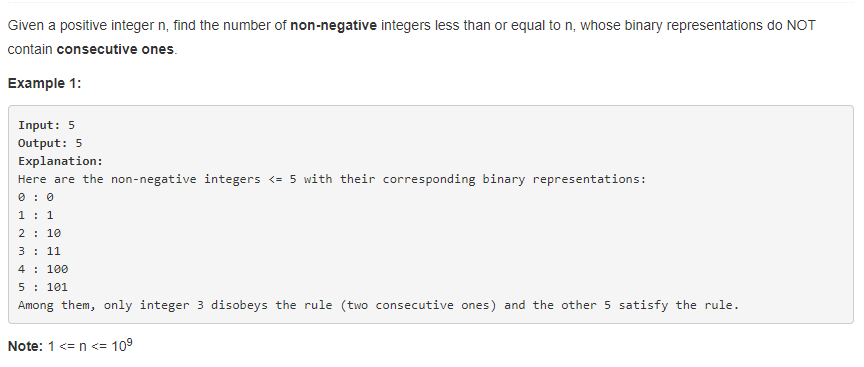
\includegraphics[width=15cm]{600.png}
		\end{center}
	\end{figure}
	\textbf{\large{Note:}}
	\par
	\vspace{0.5em}
	\noindent
	\begin{CJK*}{UTF8}{gbsn}
		如果没有连续1出现,那么这个可能的数字中肯定不会包含0x11\textellipsis,所以假设对于有\textit{n}个比特的正整数来说,其范围是从 $0 \to \underbrace{11\mathellipsis 1}_{n}$。符合题目要求的数字范围为两个部分
		\begin{enumerate}
			\item $10\underbrace{0\mathellipsis0}_{k-2} \to 10\underbrace{11\mathellipsis1}_{k-2}$,即头两位为1和0的数字
			\item $0\underbrace{00\mathellipsis0}_{k-1} \to 0\underbrace{11\mathellipsis1}_{k-1}$,即第一位为0的数字
		\end{enumerate}
		由于剩下的数字都会以11开头,所以都要舍弃。假设$DP(n)$为\textit{n}个比特的正整数中不连续1的数字个数,根据上述分析,我们有如下递推公式
		\[
		DP(n) = DP(n-2)+DP(n-1)
		\]
		而$DP(1)=2$, $DP(2)=3$,典型的Fibnocci公式。题目中是正整数,所以比特位最大为31。
		\par
		给定任何一个整数,我们先得到他的二进制表达式,然后对其中出现的每一个bit 1, 计算出其右边的bit位数。以数字100举例, 100的二进制为 1100100,
		\begin{enumerate}
			\item 其最高位的1, 其右边有6位,那么其所有的不大于100的没有连续bit 1的数字个数就等于$DP(6)$.即从
			$$
			0\underbrace{000000}_{6} \rightarrow 0\underbrace{111111}_{6}
			$$
			这些数字中选择。
			\item 接下来第6个bit位也是1, 其右边有5位,可选择的数字范围即为
			$$
			10\underbrace{00000}_{5} \rightarrow 10\underbrace{11111}_{5}
			$$
			即$DP(5)$
			\item 接下来就没有了,为什么?因为发现已经出现了两个连续的1了。后面可选择的数字肯定都要以11开头的。所以最终结果就是$DP(5)+DP(6)$
		\end{enumerate}
		所以在实现的时候,如果出现了两个连续1,我们直接返回已经得到的结果,如果一直没有出现,我们需要在得到的结果上加1,因为这个数本身也是符合条件的。
		
		\clearpage
	\end{CJK*}

\subsection{605 -- Can Place Flowers}
\begin{figure}[H]
	\begin{center}
		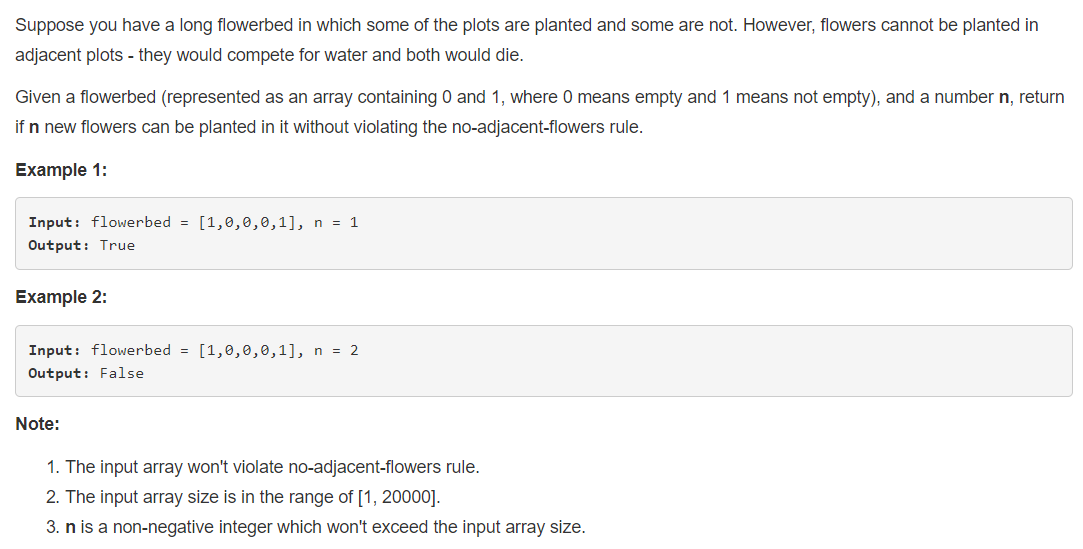
\includegraphics[width=15cm]{605.png}
	\end{center}
\end{figure}
\textbf{\large{Note:}}
\par
\vspace{0.5em}
\noindent
\begin{CJK*}{UTF8}{gbsn}
	\begin{itemize}
		\item 基本思想: 计算出连续0的子序列,如果这个子序列长度$L$大于等于3, 就可以种花最多的位置个数为(L-2+1)/2,$L-2$是因为两端的0是不能种花的。因为和1相邻。
		\item 有两个边界情况需要特殊处理:
		\begin{enumerate}
			\item 数组元素全部为0。 在这种情况下, 可以种花的最多位置为$(L+1)/2$. $L$是因为两端都能种花。
			\item 子序列的边界就是原数组的左边界或者是右边界。这种情况下,可以种花的最多位置为$(L-1+1)/2$. $L-1$是因为有一端是不能种花的。
		\end{enumerate} 
	\end{itemize}
\clearpage
\end{CJK*}

\subsection{606 -- Construct String from Binary Tree}
\begin{figure}[H]
	\begin{center}
		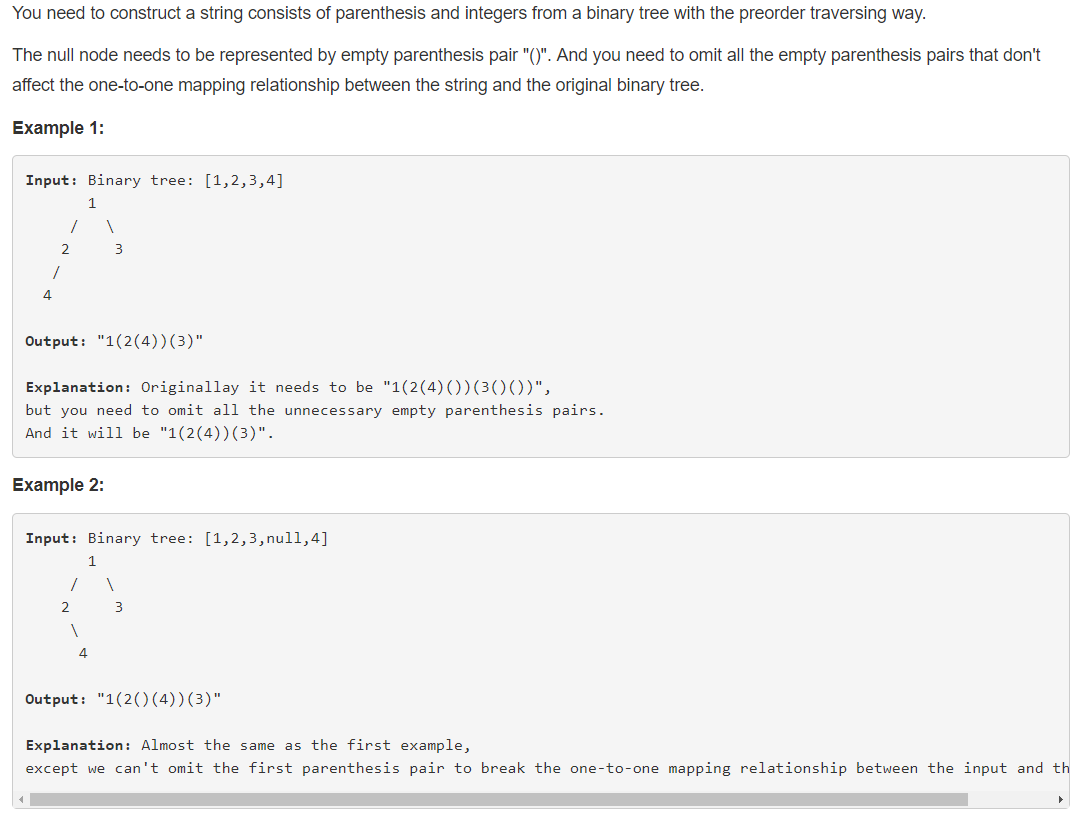
\includegraphics[width=15cm]{606.png}
	\end{center}
\end{figure}
\textbf{\large{Note:}}
\par
\vspace{0.5em}
\noindent
\begin{CJK*}{UTF8}{gbsn}
	\begin{itemize}
		\item 如果当前node的left child为null, 而right child不是null,这时,left child所生成的()是不能忽略的。
		\item 否则的话, 在preorder中,先访问当前node, 然后加上一个open parenthesis$($, 然后在当前node的left继续preorder, 结束后,加上close parenthesis$)$。
		\item 接着如果当前node的right child不为null,则类似, 先加上一个open parenthesis$($, 然后在当前node的right继续preorder, 结束后,加上close parenthesis$)$。
	\end{itemize}
	\clearpage
\end{CJK*}

\subsection{609 -- Find Duplicate File in System}
\begin{figure}[H]
	\begin{center}
		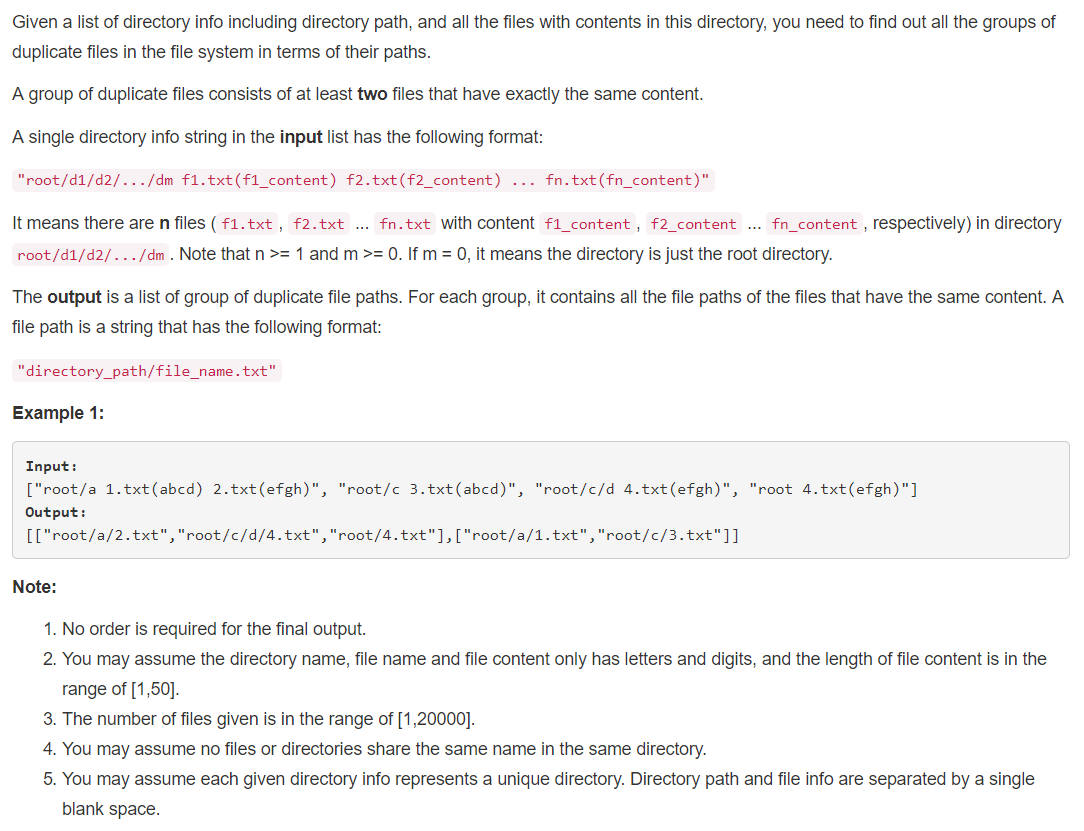
\includegraphics[width=15cm]{609.png}
	\end{center}
\end{figure}
\textbf{\large{Note:}}
\par
\vspace{0.5em}
\noindent
\begin{CJK*}{UTF8}{gbsn}
	\begin{itemize}
		\item 用一个二维vector(vector(vector(string)))来保存同一个content所对应的path列表
		\item 建立一个hashmap,key为content,value为所得到的path所在的数组在二维数组中的位置。把相同内容的path方瑞对应的数组中。
		\item 最后把只有一个元素的vector(string)去除掉。
	\end{itemize}
\clearpage
\end{CJK*}
\begin{enumerate}
	\item \textbf{Imagine you are given a real file system, how will you search files? DFS or BFS?}
	\par
	In general, BFS will use more memory then DFS. However BFS can take advantage of the locality of files in inside directories, and therefore will probably be faster
	\item \textbf{If the file content is very large (GB level), how will you modify your solution?}
	\par
	In a real life solution we will not hash the entire file content, since it's not practical. Instead we will first map all the files according to size. Files with different sizes are guaranteed to be different. We will than hash a small part of the files with equal sizes (using MD5 for example). Only if the md5 is the same, we will compare the files byte by byte.
	\item \textbf{If you can only read the file by 1kb each time, how will you modify your solution?}
	\par
	This will not change the solution. We can create the hash from the 1kb chunks, and then read the entire file if a full byte by byte comparison is required.
	\item \textbf{What is the time complexity of your modified solution? What is the most time-consuming part and memory consuming part of it? How to optimize?}
	\par
	Time complexity is O($n^2 * k$) since in worse case we might need to compare every file to all others. k is the file size
	\item\textbf{ How to make sure the duplicated files you find are not false positive?}
	\par
	We will use several filters to compare: File size, Hash and byte by byte comparisons.
\end{enumerate}

\section{610 -- 619}

\subsection{611 -- Valid Triangle Number}
\begin{figure}[H]
	\begin{center}
		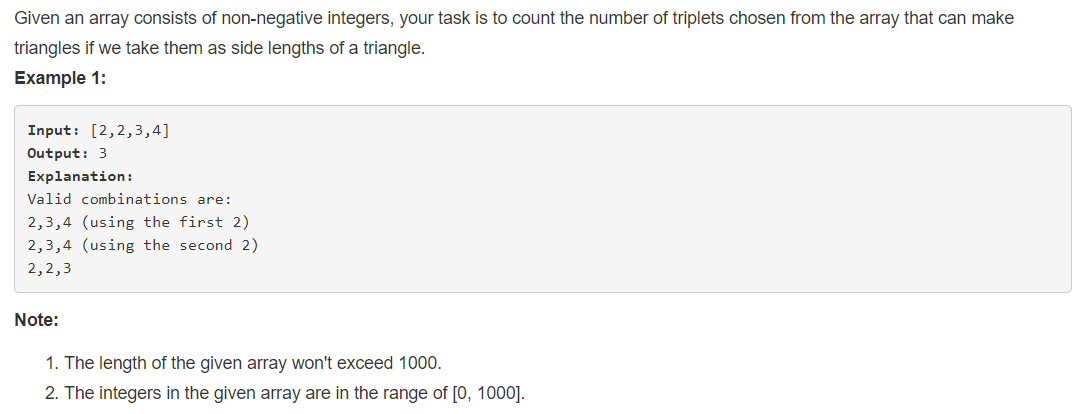
\includegraphics[width=15cm]{611.png}
	\end{center}
\end{figure}
\textbf{\large{Note:}}
\par
\vspace{0.5em}
\noindent
\begin{CJK*}{UTF8}{gbsn}
	\begin{itemize}
		\item 首先需要对数组$A$进行排序。
		\item 从倒数第二个数即$i = \text{LEN} -2 $ 开始往前遍历,假设$L=0$, $R=i-1$。最外侧循环我们把$i$从$L-1$一直循环到2. 因为三角形需要三个边,所以至少需要三个数组元素。
		\item 接着进入到内部循环寻找两个边大于$A[i]$的个数。
		\item 如果$A[L] + A[R] > A[i]$, 那么数组$A$中, 从$L$到$R-1$, 和$A[R]$相加都会大于$A[i]$, 因为$A[L]$是最小的。所以符合要求的个数为$(R-1)-L +1 = R - L$。然后$R$减1。
		\item 如果$A[L] + A[R] \leq A[i]$,那么$A[L]$还是有点小,需要增大$A[L]$, 所以$L$加1。
		\item 如果$L \ge R$, 那么就结束本次寻找,继续外部循环
	\end{itemize}
	\clearpage
\end{CJK*}

\subsection{617 -- Merge Two Binary Trees}
\begin{figure}[H]
	\begin{center}
		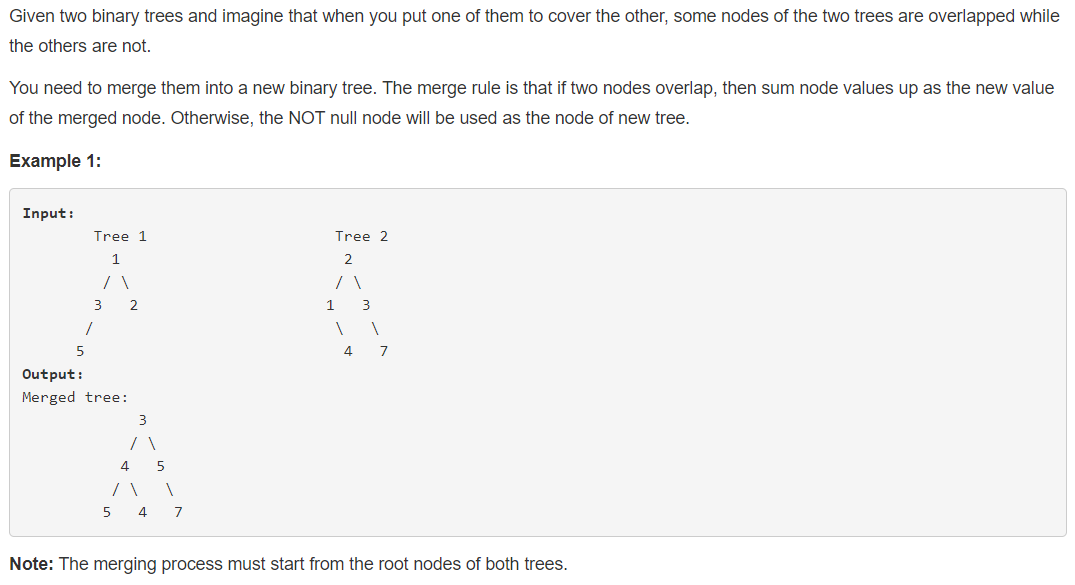
\includegraphics[width=15cm]{617.png}
	\end{center}
\end{figure}
\textbf{\large{Note:}}
\par
\vspace{0.5em}
Use recursive method. We apply the function at $t_1$'s left with $t_2$'s left, and $t_1$'s right with $t_2$'s right. There are 3 boundaries to be taken care.
\begin{itemize}
	\item $t_1$ is empty and $t_2$ is empty, we just return empty.
	\item $t_1$ is not empty but $t_2$ is empty, return $t_1$.
	\item $t_1$ is empty but $t_2$ is not, return $t_2$.
	\item In other cases, we first replace $t_1$'s value by the sum of values of $t_1$ and $t_2$. Then we just let $t_1$'s left equal to the merge of $t_1$'s left and $t_2$'s left, and $t_1$'s right equal to the merge of $t_1$'s right and $t_2$'s right. Return $t_1$.
\end{itemize}

\section{620 -- 629}
\subsection{621 -- Task Scheduler}
\begin{figure}[H]
	\begin{center}
		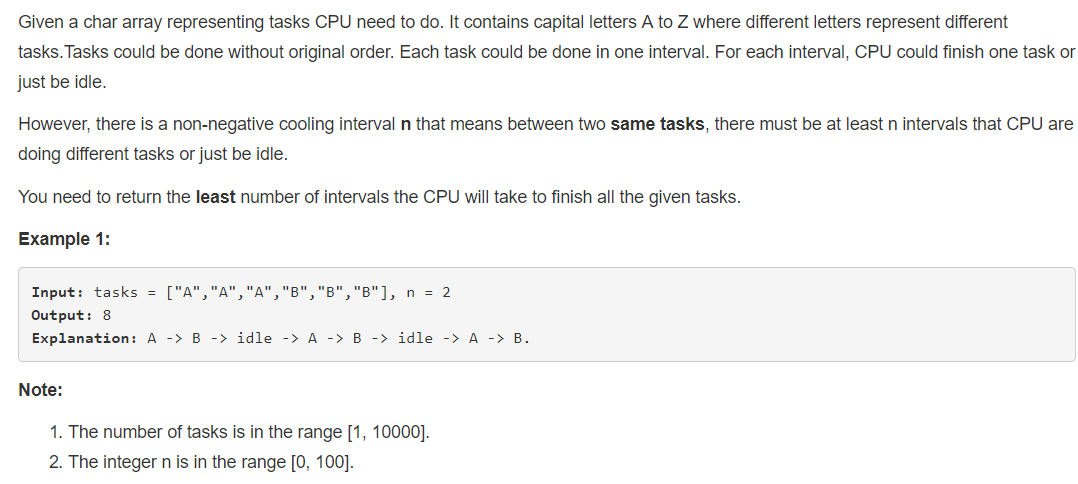
\includegraphics[width=18cm]{621.png}
	\end{center}
\end{figure}
\textbf{\large{Note:}}
\par
\vspace{0.5em}
\noindent
\begin{CJK*}{UTF8}{gbsn}
	有两种方法,一个是基于可产生的slot分析,另一个是用程序的方式,不管哪种方法,其本质都是基于greedy search。第一种方法如下:
	\begin{itemize}
		\item 假设$A$是所有任务中出现频率最高的,那么我们应当基于$A$来进行任务安排。例如,假设任务列表为$3A$, $2B$和$1C$, 而$n=2$。 那么我们先把安排$A$, 然后在两个$A$中间插入B和C, 就得到$ABC|AB\star|A$.
		\item 所以denote出现最高频率的task的总数为$K$,那么这$n$个task点之间就会有$K-1$个$slots$,每个slot之间的task和可能的idle的总数为$n-1$.
		$$
		A\underbrace{\ldots}_{n}A\ldots A\underbrace{\ldots}_{n}A\ldots A
		$$
		\item 这时候会发现,如果task种类$T$小于$n$, idle的个数就为$n-T$.因为我们可以在每一个slot把每个种类的一个task放进去,然后再放idle。所以最终需要的CPU cycyles为
		$$
		(K-1)\times n
		$$
		\item 如果task种类$T$大于$n$,这时候就不需要idle了, 只需要把所有种类的task按照一个个放入slot中,这样由于slot中所有种类的task数量已经超越$n$了, 自然也就符合题目的要求。
		\item 所以无论是那种情况,我们所能得到的最短cycle数都是
		$$
		(K-1)\times n
		$$
		但是这只是最高频率的task只有一种的情况下。
		\item 如果具有最高频率的task有多个,我们可以把这些task一个个串起来,比如,$3A$, $3B$, $2C$, $1D$, $n=3$,我们可以按照如下安排
		$$
		ABCD|ABC\star|AB\star|AB
		$$
		把$AB$当作一个task
		$$
		(AB)CD|(AB)C\star|(AB)\star|(AB)
		$$
		这与只有$A$是最高频率的task类似,只不过可用的slot从3变成了2, 因为多了一个$B$.
		\item 由于其他非最大数量的task有可能在最后一个gap之前就用完了,所以需要通过计算总的slot个数以及可用于task的slot总的个数进行分析,而不是单独对一个gap进行分析。首先要得到在gap中间需要需要放入多少个slots,这个slots可能包含task和idle,取决于task的数量,所以需要计算总数,而不是单独的gap中的task。例如$4A$, $4B$, $2C$, $n=3$,那么根据分析有
		$$
		ABC\star|ABC\star|AB\star\star|AB
		$$
		在最后一个gap, task C就没有了,已经用完了,需要填入idle。但是总的slots仍然是
		$$
		\texttt{gaps}\times \texttt{n - (\texttt{number of maximum tasks - 1)}} = 3 \times(3 - (2-1))=6
		$$
		这里需要把$AB$当作一个整体,因为他们具有相同数量而且都是最大数量的task。
	
		\begin{enumerate}
			\item $R = \texttt{number of unique tasks with maximum count}$
			\item $G = \texttt{total gaps}$
			\item $M = \texttt{count of the task which appear most frequently}$
			\item $G = M - 1$
			\item $S = \texttt{total count of tasks which do not appear most often}$
			\item $T = \texttt{total count of tasks}$
			\item $S = T - R \times M$
			\item $L = \texttt{total slots need to inserted in all gaps}$\
			\item $L = G \times (n - (R-1))$
			\item $I = \texttt{total idles needed}$
			\item  $I = \max(0, L - S)$
			\item $N = \texttt{minimum total cycles}$
			\item $N = T + I$
		\end{enumerate}
	
	$$
	\underbrace{AB}_{R}\overbrace{\underbrace{CDE\ldots}_{S_{1}}\underbrace{\star\star\ldots}_{I_{1}}}^{n}AB\ldots AB\overbrace{\underbrace{CDE\ldots}_{S_{G}}\underbrace{\star\star\ldots}_{I_{G}}}^{n}AB
	$$
	在这里,$\sum\limits_{i=1}^{G}S_{i} = S$, $\sum\limits_{i=1}^{G}I_{i} = I$以及$S+I = L$
	\end{itemize}
\clearpage
\end{CJK*}

\subsection{622 -- Design Circular Queue}
\begin{figure}[H]
	\begin{center}
		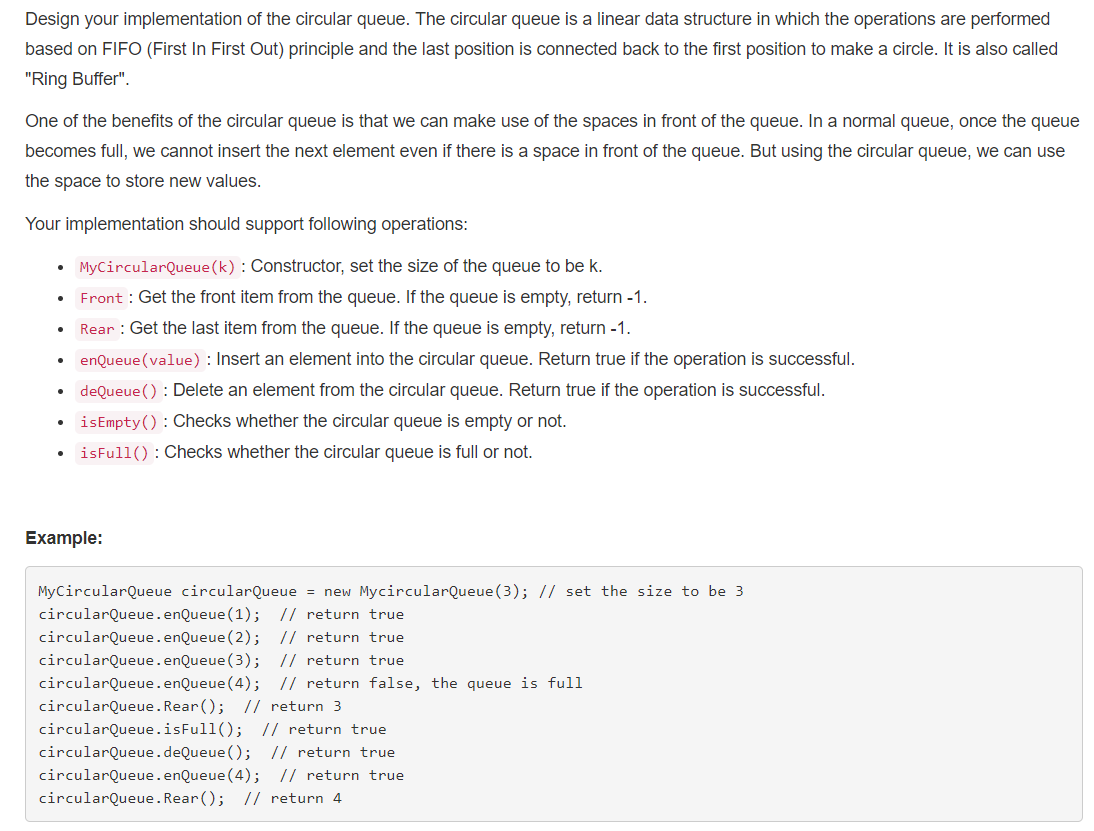
\includegraphics[width=18cm]{622.png}
	\end{center}
\end{figure}
\textbf{\large{Note:}}
\par
\vspace{0.5em}
\begin{itemize}
	\item Requires the following members
	\begin{enumerate}
		\item \texttt{len} --- The current number of elements in the queue.
		\item \texttt{head} --- The head index of the queue. When dequeue one element, 
		$$
		\texttt{head} = (\texttt{head + 1}) \% \texttt{len}
		$$
		\item \texttt{cap} --- The maximum capacity of the queue
		\item \texttt{tail} --- The tail index of the queue. When insert an element
		$$
			\texttt{tail} = (\texttt{tail + 1}) \% \texttt{len}
		$$
	 \end{enumerate}
 \item When decide if the queue is empty or full, simply check if $\texttt{len} = \texttt{0}$ or $\texttt{len} = \texttt{cap}$
\end{itemize}

\subsection{623 -- Add One Row to Tree}
\begin{figure}[H]
	\begin{center}
		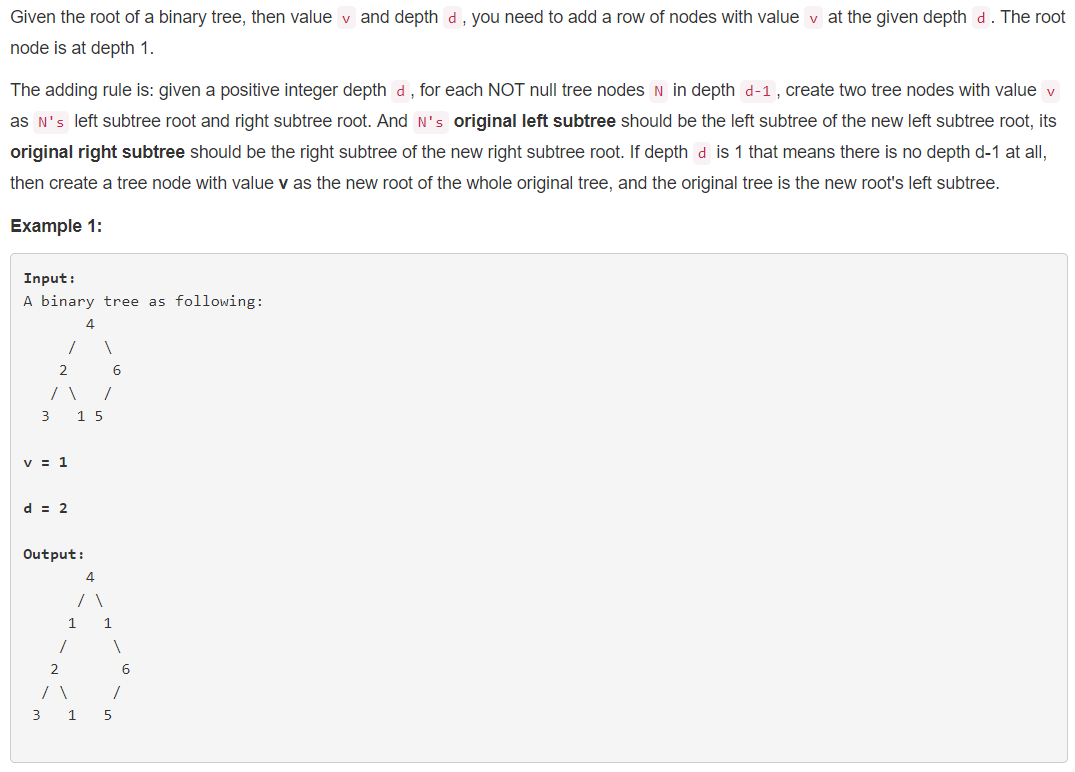
\includegraphics[width=18cm]{623_1.png}
	\end{center}
\end{figure}
\begin{figure}[H]
	\begin{center}
		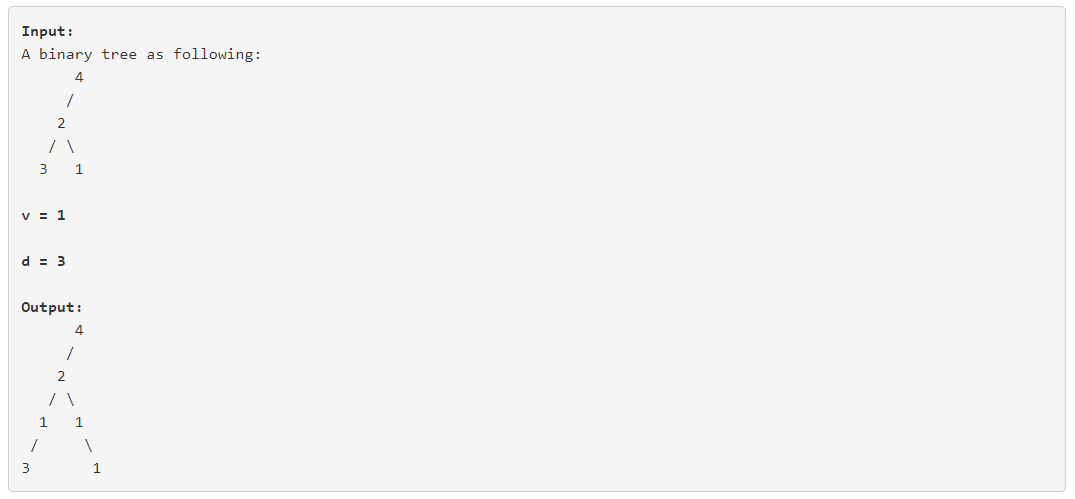
\includegraphics[width=18cm]{623_2.png}
	\end{center}
\end{figure}
\textbf{\large{Note:}}
\par
\vspace{0.5em}
\begin{itemize}
	\item This is a easy problem. Using recursive method, provide a recursive function with \texttt{node}, $d$, $v$ and \texttt{cur\textunderscore level} as the input parameters
	\item if $\texttt{cur\textunderscore level} = d - 1$, then for each non null node:
	\begin{enumerate}
		\item save its left and right subtree first, and then create left and right subtree with $v$. 
		\item assign the saved left subtree to \texttt{left child} of the new created left subtree and the saved right substree to \texttt{right child} of the new create right subtree.
	\end{enumerate}
	\item otherwise, recursive call the function on current node's left subtree if it is not null with $\texttt{cur\textunderscore level} + 1$. Same for the current node's right subtree.
	\item if $d=1$, create a new root node as require and assign \texttt{root} as the \texttt{left child} of the new root node.
\end{itemize}

\subsection{624 -- Maximum Distance in Arrays}
\textbf{\Huge{TODO}}

\subsection{625 -- Minimum Factorization}
\textbf{\Huge{TODO}}

\subsection{628 -- Maximum Product of Three Numbers}
\begin{figure}[H]
	\begin{center}
		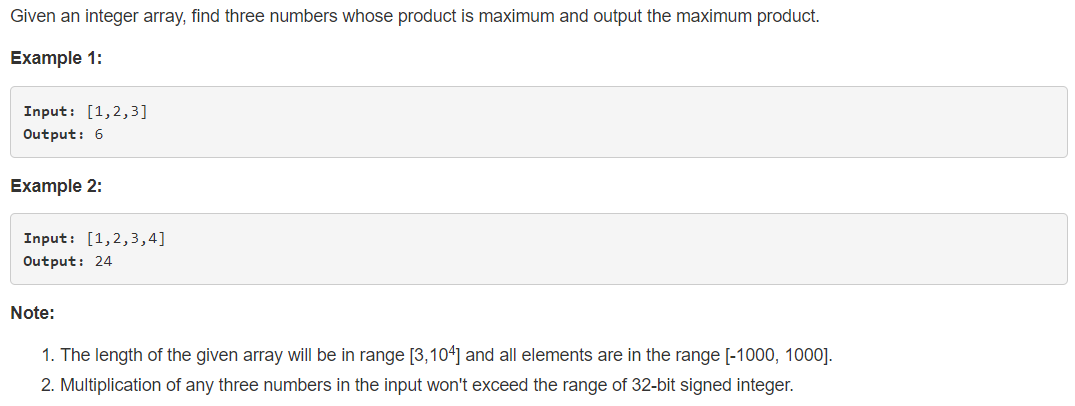
\includegraphics[width=18cm]{628.png}
	\end{center}
\end{figure}
\textbf{\large{Note:}}
\par
\vspace{0.5em}
\begin{CJK*}{UTF8}{gbsn}
	\begin{itemize}
		\item 由于可能有负数,所以需要找到三个最大的整数,和两个最小的负数,然后比较两个负数和最大整数的product,与三个整数的product的大小。
	\end{itemize}
	\clearpage
\end{CJK*}	

\subsection{629 -- K Inverse Pairs Array}
\begin{figure}[H]
	\begin{center}
		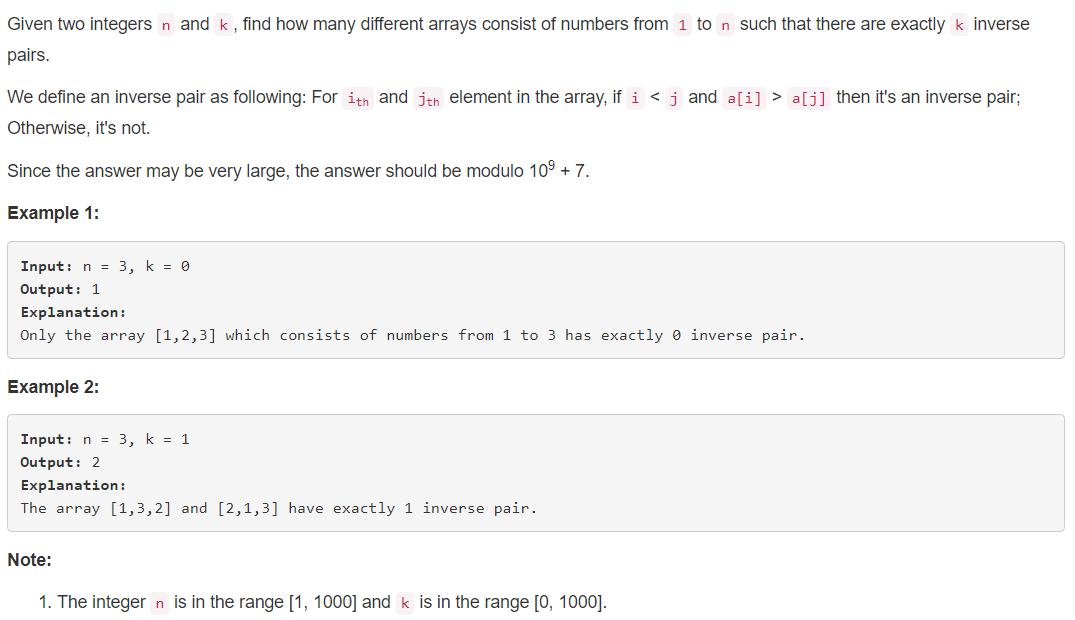
\includegraphics[width=18cm]{629.png}
	\end{center}
\end{figure}
\textbf{\large{Note:}}
\par
\vspace{0.5em}
\noindent
\begin{CJK*}{UTF8}{gbsn}
	\begin{itemize}
		\item 采用DP方式,找到recursive equation $\mathtt{dp}(n, k)$, 即从$1\to n$, 有k个\texttt{inverse pairs}的数列个数。
		\item 为了找到recursive equation,分析从$n-1$变换到$n$时,\texttt{how many more inverse pairs are added}.
		\begin{enumerate}
			\item 如果新增的$n$在位置$n$,那么由于$1 \to n$中没有数能比$n$大,所以,在这个位置放n,不会产生新的\texttt{inverse pair}. 所以这时候的有$k$个inverse pairs的array个数仍然是$\mathtt{dp}(n-1, k)$
			\item 如果$n$放在位置$n-1$,由于位置$n$必然被$1 \to n-1$中的任何一个数所占据,所以把$n$放在位置$n-1$上的数组中的任何一个都会由于$n$而产生一个\texttt{inverse pair},那么另外$k-1$个\texttt{inverse pair}就要靠安排剩下的$1\to n-1$产生了。所以这时候有$k$个\texttt{inverse pair}的array个数则是$\mathtt{dp}(n-1, k-1)$;
			\item \ldots
			\item 如果$n$放在位置$1$, 由于位置$2 \to n$必然被$1 \to n-1$的所有数所占据,所以把$n$放在位置1上的数组中的任何一个都会由于$n$而产生$n-1$个\texttt{inverse pair},那么剩下的$k-(n-1)$个\texttt{inverse pair}就要靠安排剩下的$1\to n-1$产生了。所以这时候有$k$个\texttt{inverse pair}的array个数则是$\mathtt{dp}(n-1, k-(n-1))$。(注意:这里没有考虑k和n的大小关系,k可能小于或者远小于n-1,所以有的k实际上不会recursive到这里的,在实现的时候需要考虑)。
			\item 最后总结得到的recursive equation:
			$$
			\mathtt{dp}(n, k) = \mathtt{dp}(n-1, k) + \mathtt{dp}(n-1, k-1) + \ldots + \mathtt{dp}(n-1, k-(n-1))
			$$
		\end{enumerate}
	\item 如果直接用上述recursive equation, 仍然效率不是很高。通过观察equation中$dp(n, k-1)$,由于
	$$
	\mathtt{dp}(n, k-1) = \mathtt{dp}(n-1, k-1) + \mathtt{dp}(n-1, k-2) + \ldots + \mathtt{dp}(n-1, k-1-(n-2)) + \mathtt{dp}(n-1, k-1-(n-1))
	$$
	于是结合两个equation,可以得到如下equation
	\begin{equation}
	\begin{split}
	\mathtt{dp}(n, k) &= \mathtt{dp}(n-1, k) + \underbrace{\mathtt{dp}(n-1, k-1) + \ldots + \mathtt{dp}(n-1, k-(n-1))}_{\texttt{could be part of }\mathtt{dp}(n, k-1)} \\
	&= \mathtt{dp}(n-1, k) + \underbrace{\mathtt{dp}(n-1, k-1) + \ldots + \mathtt{dp}(n-1, k-(n-1)) + \mathtt{dp}(n-1, k-n)}_{\mathtt{dp}(n, k-1)} \\
	&\qquad \qquad - \mathtt{dp}(n-1, k-n) \\
	&= \mathtt{dp}(n-1, k) + \mathtt{dp}(n, k-1) - \mathtt{dp}(n-1, k-n)
	\end{split}
	\end{equation}
	\item 在实现的时候,\texttt{dp}的\texttt{size}为$(n+1)\times(k+1)$, $k=0$时, 都为1, 然后初始以$n=3$开始,因为$\mathtt{dp}(2,1)=1$。$\mathtt{dp}(n-1, k-n)$只有当$k \geq n$的时候才会被减掉。
	\end{itemize}
	\clearpage
\end{CJK*}


\section{630 --- 639}
\subsection{630 -- Course Schedule III}
\begin{figure}[H]
	\begin{center}
		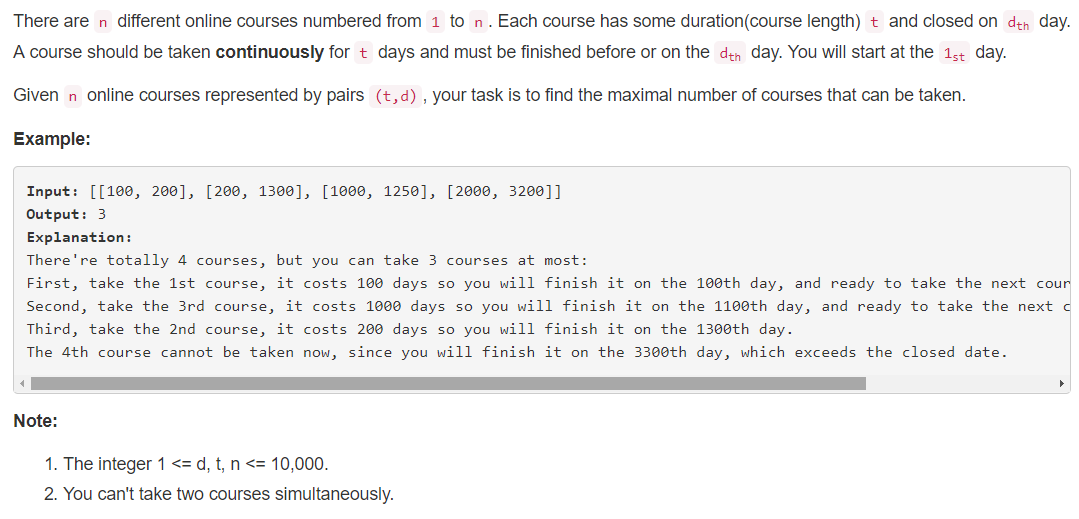
\includegraphics[width=18cm]{630.png}
	\end{center}
\end{figure}
\begin{CJK*}{UTF8}{gbsn}
	\begin{itemize}
		\item 基于Greedy Method, 首先按照close day有低到高排序。
		\item Next, 用一个max priority queue里面的node是各个course的duration。然后set 时间总和$T$为$0$.
		\item 从第一个course开始,把当前course的duration放入queue中。如果该course的duration加上到目前为止的$T$小于course的close time, 则继续到下一个course。
		\item 如果超过了close time,这时候我们需要从queue中remove一个course,那么哪个course是最佳候选呢,很显然,duration越大的越应该移除(Greedy)。而queue的top刚好就是这个需要移除的durtaion。 所以把这个duration从$T$中移除。
		\item 最后,queue中的node个数就是需要的答案了。
	\end{itemize}
\clearpage
\end{CJK*}

\subsection{631 -- Design Excel Sum Formula}
\textbf{\Huge{TODO}}

\subsection{632 -- Smallest Range}
\begin{figure}[H]
	\begin{center}
		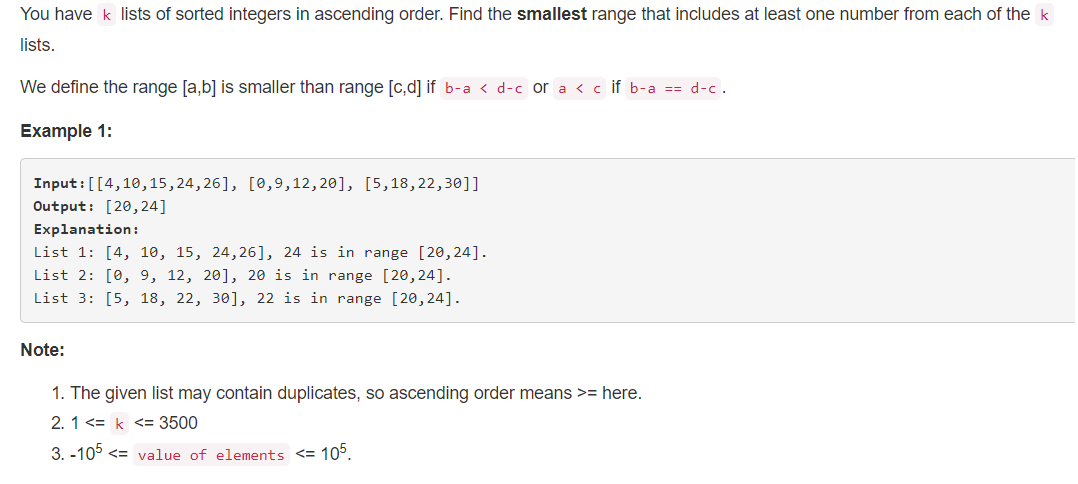
\includegraphics[width=18cm]{632.png}
	\end{center}
\end{figure}
\textbf{\large{Note:}}
\par
\vspace{0.5em}
\noindent
\begin{CJK*}{UTF8}{gbsn}
	\begin{itemize}
		\item Basic idea: 用一个min priority\textunderscore queue,其内部节点结构为\texttt{pair\textless size\textunderscore t, size\textunderscore t\textgreater},其中\texttt{pair.first}代表当前数字所在数组在输入的二维数组中的\texttt{index},\texttt{pair.second}则代表当前输在在其所在数组中的\texttt{index}。通过使用这种方法,把\textbf{queue}中的node和输入的二维数组联系起来,而不再是单纯的数字了。另外一种方法使用\textbf{iterator},这里采用第一种方法。
		\item 首先把各个数组的第一个数字放入\textbf{queue}中,这样在\textbf{queue}中我们都有一个来自各数组的数字。同时需要获得这些数字的最大值$H$和最小值$L$,以此作为最终\texttt{range}的初始上限和下限
		\item 接着开始用\textbf{queue}是否为\textbf{empty}作为循环退出的条件。在循环中,从\textbf{queue}中弹出并得到\textbf{top}元素,该元素按照前面的设计,是一个\textbf{pair},我们将其\textbf{second}加1,也就是当前这个数字$M$所在数组的下一个数字在当前这个数字所在数组的\texttt{index}。如果这个\textit{index}已经和当前这个数字所在数组的长度相等了,表示已经扫描完了这个数组了,这个时候也需要退出循环。因为题目要求是\texttt{range}中包含每个数组中的至少一个数字。如果不退出,可能以后更新的\texttt{range}就不会包含当前这个数字所在数组的数字了(因为已经扫描完了)。
		\item 如果还在当前数字$M$所在数组的范围内,我们将这个数字$N$也就是当前数字$M$所在数组中的下一个数字的坐标放入\textbf{queue}中。这是因为我们从原来的\textbf{queue}中\textbf{remove}掉当前的这个数字,也就是说再放入这个数字$N$之前\textbf{queue}中没有了当前数字所在数组的数字了。这时候,需要更新当前\texttt{range}的下限为\textbf{queue}的top元素。因为这时候top元素可能由于新加入的最新数字而发生了改变。这时候有两种情况
		\begin{enumerate}
			\item 加入的数字$N$是最小的,那么当前\texttt{range}需要更新为$N$。
			\item 如果不是,那么当前\texttt{range}需要更新为去除top元素之后的最小元素。
		\end{enumerate}
	无论发生哪种情况,当前的\texttt{range}都需要做更新。同时把$R$更新为$R$和$N$的最大值。这样更新后的\texttt{range}同样包含了每个数组中的至少一个数字。只不过是把$M$替换为了$N$.
	\item 之所以上限$R$需要比较,而下限$L$不需要比较,是因为下限$L$已经通过priority\textunderscore queue的操作已经是最小的了。
	\item 最后比较$R$与$L$是否是当前最小的\textit{range}。接着继续循环。
	\end{itemize}
	\clearpage
\end{CJK*}

\subsection{634 -- Find the Derangement of An Array}
\textbf{\Huge{TODO}}

\subsection{635 -- Design Log Storage System}
\textbf{\Huge{TODO}}

\subsection{636 -- Exclusive Time of Functions}
\begin{figure}[H]
	\begin{center}
		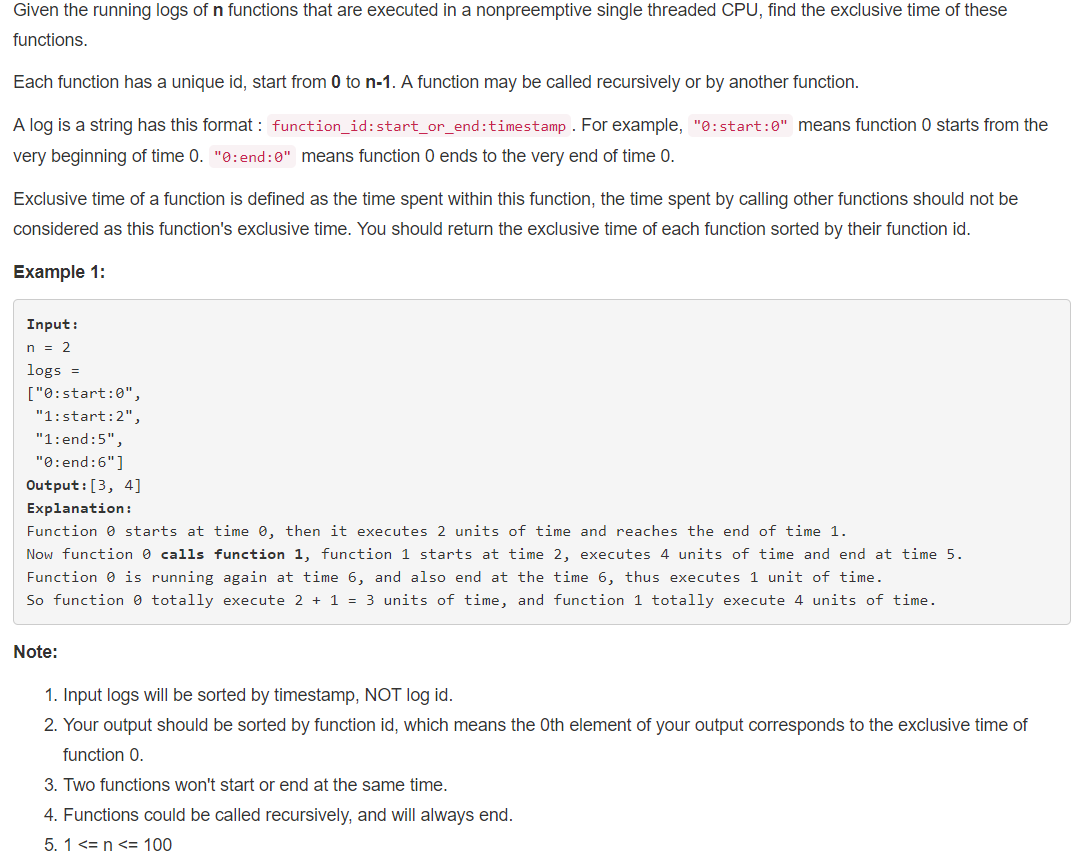
\includegraphics[width=18cm]{636.png}
	\end{center}
\end{figure}
\textbf{\large{Note:}}
\par
\vspace{0.5em}
\begin{itemize}
	\item Since each task will reduce the contained tasks' running time, use a \textbf{stack} to record the latest \texttt{id}.
	\item At the beginning, parse the \textbf{first} log. Push the \texttt{id} into the stack. Also, save the time as \textit{prev}.
	\item Start the loop from the second log.
	\begin{itemize}
		\item if the log is \textbf{start}, 
		\begin{enumerate}
			\item First, add the running time of the \texttt{id} which is the top of the stack with the difference of the current time and \textit{prev}.
			\item Next, push current \texttt{id} into the stack and update \textit{prev} as the current time.
		\end{enumerate}
		\item otherwise, this log contains the information of task \textbf{ending}.
		\begin{enumerate}
			\item First, we add the running time of the  \texttt{id} which is the top of the stack with the difference of the current time and \textit{prev}, also need to add $\mathbf{(1)}$ since the end of current time needs to be considered.
			\item Next, pop the top \texttt{id} from the stack. Also, update \textit{prev} as the current time plus $\mathbf{(1)}$ since this is the end of the current time.
		\end{enumerate}
	\end{itemize}
\end{itemize}

\subsection{637 -- Average of Levels in Binary Tree}
\begin{figure}[H]
	\begin{center}
		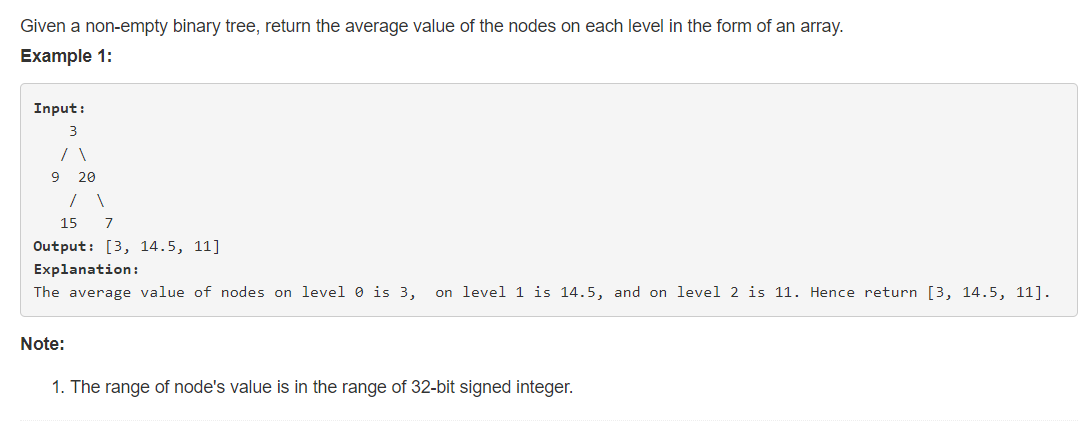
\includegraphics[width=18cm]{637.png}
	\end{center}
\end{figure}
\textbf{\large{Note:}}
\par
\vspace{0.5em}
\begin{itemize}
	\item An easy problem: use a queue and for each level, get the current size of the queue and pop each node from the queue.
	\item Need to take consideration of possible overflow. Therefore, each level's sum will be \texttt{double} type.
\end{itemize}

\subsection{638 -- Shopping Offers}
\begin{figure}[H]
	\begin{center}
		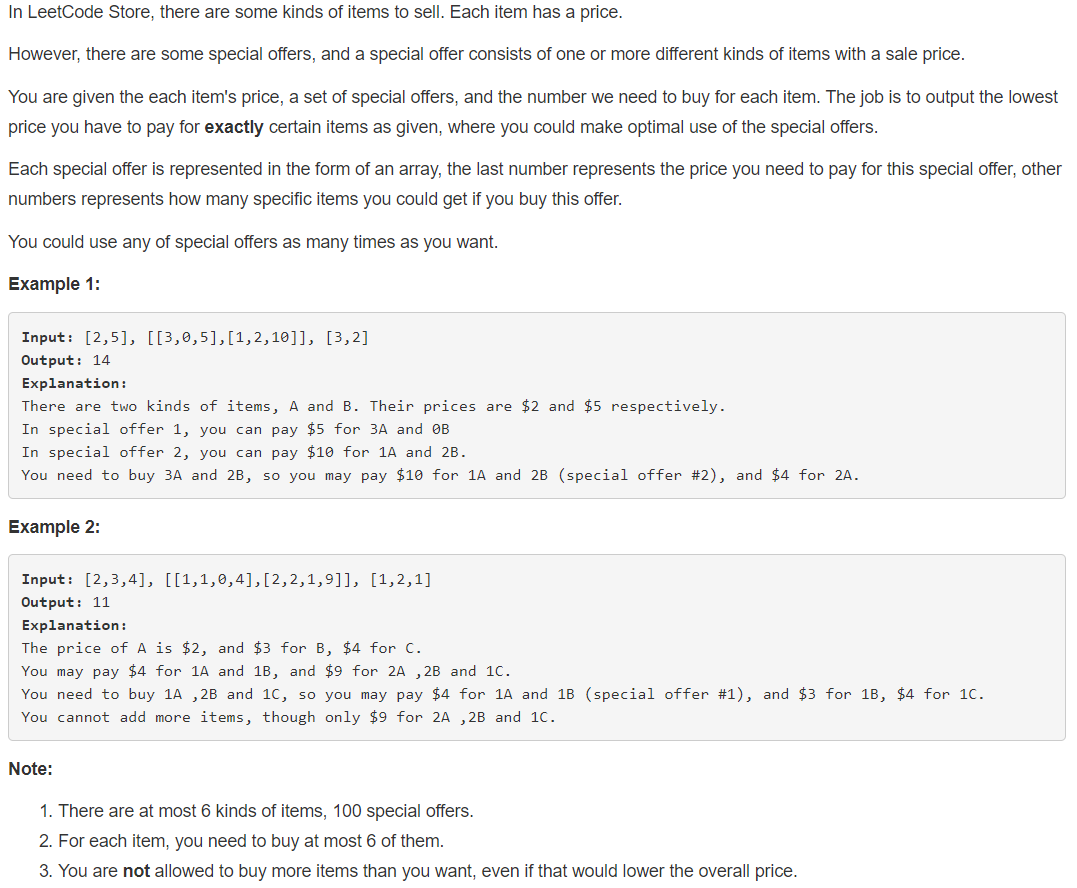
\includegraphics[width=18cm]{638.png}
	\end{center}
\end{figure}
\textbf{\large{Note:}}
\par
\vspace{0.5em}
\begin{CJK*}{UTF8}{gbsn}
	\begin{itemize}
		\item 一个special offer是否被接受,取决于当前所需的quantity是否大于等于对应的\textbf{special offer}所提供的quantity。
		\item 基于recursive原理,不难写出function的原型find\textunderscore offer(price, specials, current\textunderscore needs, start, total\textunderscore cost, minimum\textunderscore cost)。其中\texttt{current\textunderscore needs}代表recursive到current level时,还有多少需求剩余。\texttt{start}代表的是从哪个\texttt{index}开始测试\textbf{special offer}。\texttt{total\textunderscore cost}代表的是recursive到current level时,已经产生了多少cost,最后的\texttt{min\textunderscore cost}则就是需要返回的最小的cost。
		\item 在find\textunderscore offer中, 从当前start开始测试每个offer,一直到special offer的最后,首先将当前的\texttt{current\textunderscore needs}保存起来,然后测试当前special offer是否可以接受,如果不可以,需要重置\texttt{current\textunderscore needs}为保存的value,继续循环。如果被接受,则开始recursive,这时\texttt{start}为当前的可接受的special offer的\textbf{index},因为题目说同一个offer可以用多次,然后\texttt{total\textunderscore cost}更新为与当前offer的cost的sum。
		\item 接着,仍然需要重置\texttt{current\textunderscore needs}为保存的value,因为需要从下一个offer重新开始测试。
		\item 最后,循环结束后,由于\texttt{current\textunderscore needs}可能有剩余,需要在\texttt{total\textunderscore cost}加上用实际的\texttt{price}得到的\textbf{cost}。并比较最小的\textbf{cost}。
	\end{itemize}
	\clearpage
\end{CJK*}

\subsection{639 -- Decode Ways II}
\begin{figure}[H]
	\begin{center}
		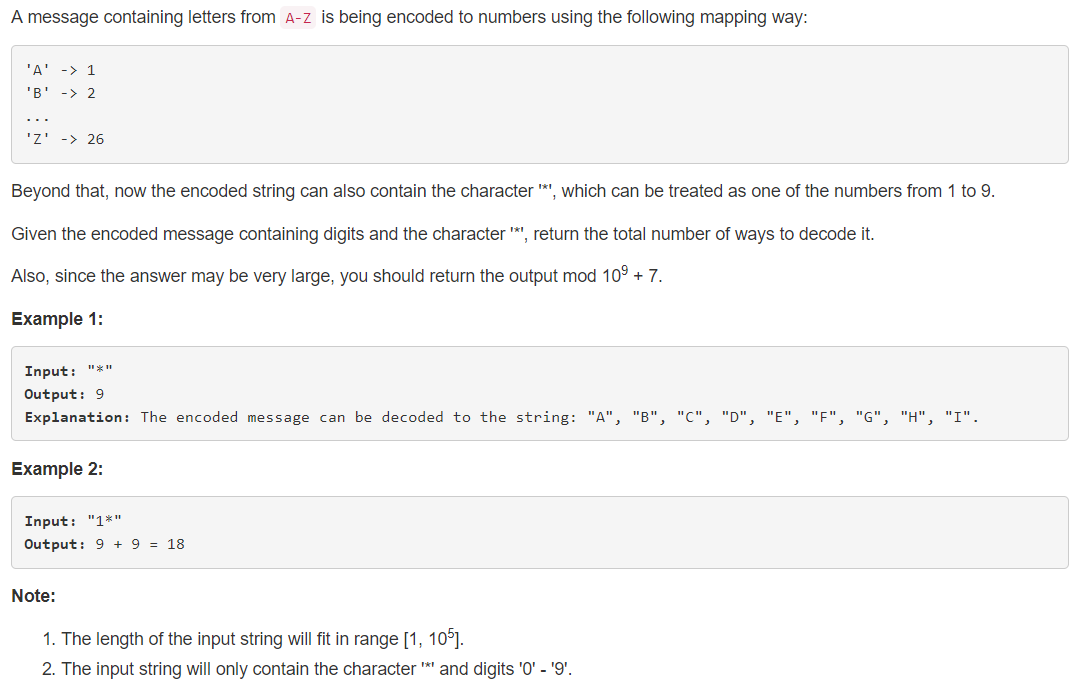
\includegraphics[width=18cm]{639.png}
	\end{center}
\end{figure}
\textbf{\large{Note:}}
\par
\vspace{0.5em}
\begin{CJK*}{UTF8}{gbsn}
	\begin{itemize}
		\item 基于\textbf{Dynamic Programming},假设当前字符\texttt{index}为$i$。 
		\item 如果$i=0$, 如果当前字符为$\star$,则有\textbf{9 ways}, 否则为\textbf{1 way}。
		\item 从第二个字符开始循环,分为三种情形。用$n_0$代表decode $S[0\mathellipsis i-2]$的ways, $n_1$代表decode $S[0\mathellipsis i-1]$的ways, $n_2$代表decode $S[0\mathellipsis i]$的ways
		\begin{enumerate}
			\item 如果为$\star$, 如果只decode这个字符,那么有9 ways,那么这时候产生的$n_2 = 9\times n_1$。但如果需要把当前这个字符和前一个字符结合起来一起decode,则有以下几种情形。
				\begin{enumerate}
					\item 如果前一个字符是2,那么因为最多只能decode 从$21\rightarrow 26$,所以总共有6 ways。所以$n2 = n_2 + n_0 \times 6$。
					\item 如果前一个字符是1,那么可以decode 从$11\rightarrow 19$, 有9 ways, 所以$n_2 = n_2 + n_0\times 9$。
					\item 如果前一个字符也是$\star$, 那么可以decode 从$11\rightarrow 19$ 和 $21\rightarrow 26$,总共$6+9=15$。 注意不会产生$20$,因为$\star$不能decode为zero。所 以$n_2 = n_2 + n_0\times 15$
					\item 如果是剩下的其他字符,都不可能decode,所以为$n_2$不变。
				\end{enumerate}		
			\item 如果为0, 那么因为0本身是不能被decode的,所以必须结合前一个字符一起进行decode。类似的,也有如下情形。
				\begin{enumerate}
					\item 前一个字符为2或者为1,只能decode $20$或者$10$,都只有one way, 所以$n_2 = n_0 \times 1$。
					\item 前一个字符为$\star$,那么$\star$能够给出的也只有1和2, 所以有2 ways, 于是$n_2 = n_0 \times 2$。
					\item 在其他情形下,都不可能decode,这时候$n_2 = n_0 \times 0 = 0$。
				\end{enumerate}
			\item 如果为其他字符,那么decode这个字符本身只有one way, 所以$n_2 = n_1 \times 1$。然后把当前这个字符和前一个字符结合起来一起decode,则一样会有以下几种情形。
				\begin{enumerate}
					\item 前一个字符为1,可以decode,但只有 one way, 所以$n_2 = n_2 + n_0 \times 1$。
					\item 前一个字符为2,这时候要看当前字符了,如果当前字符是$1 \rightarrow 6$, 那么可以decode,也是只有one way。 于是$n_2 = n_2 + n_0 \times 1$。
					\item 如果前一个字符是$\star$,同样也要看当前字符,如果当前字符也是$1 \rightarrow 6$,那么$\star$可以是1或者2,总共是2 ways,所以这时候$n_2=n_2 + n_0\times 2$。但是,如果当前字符是$ 7 \rightarrow 9$,$\star$只能是1,总共有1 way,这时候$n_2 = n_2 + n_0\times 1$。
				\end{enumerate}
		\end{enumerate}
	\item 继续到下一个字符之前,$n_0=n_1$, $n_1 = n_2$。因为只需要考虑当前的三个计数值。
	\item 最后返回$n_2$
	\item 实现的时候,最开始的$n_0$ = 1而不是0, 另外需要用\texttt{long long type} 
	\end{itemize}
	\clearpage
\end{CJK*}

\section{640 --- 649}	
\subsection{640 -- Solve the Equation}
\begin{figure}[H]
	\begin{center}
		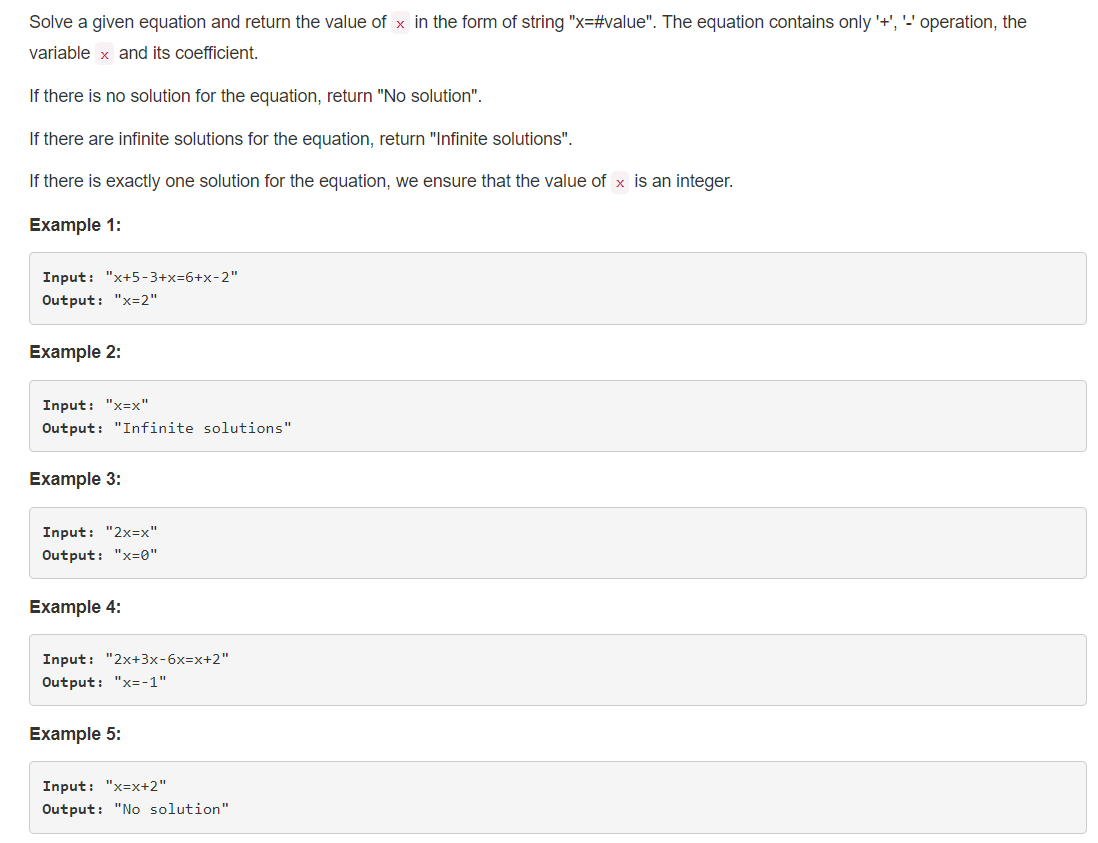
\includegraphics[width=18cm]{640.png}
	\end{center}
\end{figure}
\textbf{\large{Note:}}
\par
\vspace{0.5em}

\subsection{641 -- Design Circular Deque}
\begin{figure}[H]
	\begin{center}
		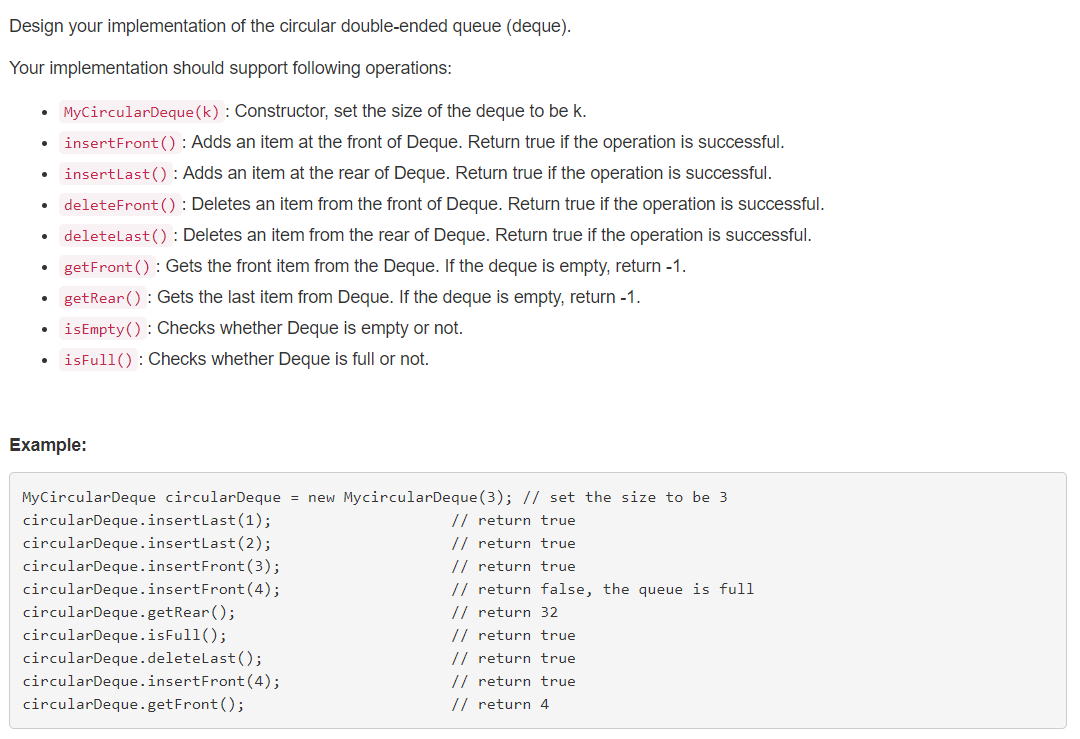
\includegraphics[width=18cm]{641.png}
	\end{center}
\end{figure}
\textbf{\large{Note:}}
\par
\vspace{0.5em}
\begin{algorithm}[H]
	\caption{Constructor}
	\label{deque-ctor}
	\begin{algorithmic}[1]
		\Procedure{CircularDequeue}{$k$}
		\State $cap := k$
		\State $size := 0$
		\State $v[k]$ \Comment typically a vector with size equal to $k$
		\State $front := 0$ \Comment \texttt{index} to the front of the deque
		\State $rear := k-1$ \Comment \texttt{index} to the rear of the deque
		\EndProcedure
	\end{algorithmic}
\end{algorithm}
	
\begin{algorithm}[H]
	\caption{Insert Element into the front}
	\label{deque-insert-front}
	\begin{algorithmic}
		\Procedure{InsertFront}{$value$}
		\If {\ref{QCheckFull}}
		\State \textbf{return} $false$ \Comment cannot insert when full
		\EndIf
		\State $size := size + 1$ \Comment number of elements increment
		\State $v[front] \gets value$ \Comment put value in \texttt{front} index.
		\State $front := (front + 1) \bmod cap$ \Comment increment \texttt{front} index
		\State \Comment need to count for the circular property of the queue
		\State \textbf{return} $true$
		\EndProcedure
	\end{algorithmic}
\end{algorithm}

\begin{algorithm}[H]
	\caption{Insert Element into the rear}
	\label{QInsertLast}
	\begin{algorithmic}
		\Procedure{InsertLast}{$value$}
		\If {\ref{QCheckFull}}
		\State \textbf{return} $false$ \Comment cannot insert when full
		\EndIf
		\State $size := (size + 1)$ \Comment number of elements increment
		\State $v[rear] \gets value$ \Comment put value in \texttt{front} index.
		\State $rear: = (rear - 1 + cap) \bmod cap$ \Comment decrement \texttt{rear}
		\State \Comment need to count for the circular property of the queue
		\State \Return $true$
		\EndProcedure
	\end{algorithmic}
\end{algorithm}

\begin{algorithm}[H]
\caption{Delete front element}
	\begin{algorithmic}
			\Procedure{DeleteFront}{}
			\If {\ref{QCheckEmpty}}
			\State \textbf{return} $false$ \Comment cannot delete when empty
			\EndIf
			\State $size := size - 1$ \Comment decrement number of elements
			\State $front := (front -1 + cap) \bmod cap$ \Comment decrement front
			\State \Comment need to count for the circular property of the queue
			\State \Return $true$
			\EndProcedure
	\end{algorithmic}
\end{algorithm}

\begin{algorithm}[H]
\caption{Delete rear element}
	\begin{algorithmic}
			\Procedure{DeleteRear}{}
			\If {\ref{QCheckEmpty}}
			\State \textbf{return} $false$ \Comment cannot delete when empty
			\EndIf
			\State $size := size - 1$ \Comment decrement number of elements
			\State $rear := (rear + 1) \bmod cap$ \Comment increment \texttt{rear}
			\State \Comment need to count for the circular property of the queue
			\State \Return $true$
			\EndProcedure
	\end{algorithmic}
\end{algorithm}

\begin{algorithm}[H]
\caption{Get front element}
	\begin{algorithmic}
			\Procedure{GetFront}{}
			\If {\ref{QCheckEmpty}}
			\State \textbf{return} $-1$ \Comment no element return when empty
			\EndIf
			\State $temp := (front -1 + cap) \bmod cap$ \Comment since \texttt{front} is in the next position
			\State \Comment need to get current element by decrement \texttt{front}
			\State \Return $v[temp]$
			\EndProcedure
	\end{algorithmic}
\end{algorithm}

\begin{algorithm}[H]
\caption{Get rear element}
	\begin{algorithmic}
			\Procedure{GetRear}{}
			\If {\ref{QCheckEmpty}}
			\State \textbf{return} $-1$ \Comment no element return when empty
			\EndIf
			\State $temp := (rear + 1) \bmod cap$ \Comment since \texttt{rear} is in the next position
			\State \Comment need to get current element by increment \texttt{rear}
			\State \Return $v[temp]$
			\EndProcedure
	\end{algorithmic}
\end{algorithm}

\begin{algorithm}[H]
\caption{Check if the queue is full}
\label{QCheckFull}
	\begin{algorithmic}
		\Procedure{IsFull}{}
		\State \Return $size \geq k$
		\EndProcedure
	\end{algorithmic}
\end{algorithm}

\begin{algorithm}[H]
\caption{Check if the queue is empty}
\label{QCheckEmpty}
	\begin{algorithmic}
		\Procedure{IsEmpty}{}
		\State \Return $size \leq 0$
		\EndProcedure
	\end{algorithmic}
\end{algorithm}

\subsection{642 -- Design Search Autocomplete System}
\textbf{\Huge{TODO}}

\subsection{643 -- Maximum Average Subarray I}
\begin{figure}[H]
	\begin{center}
		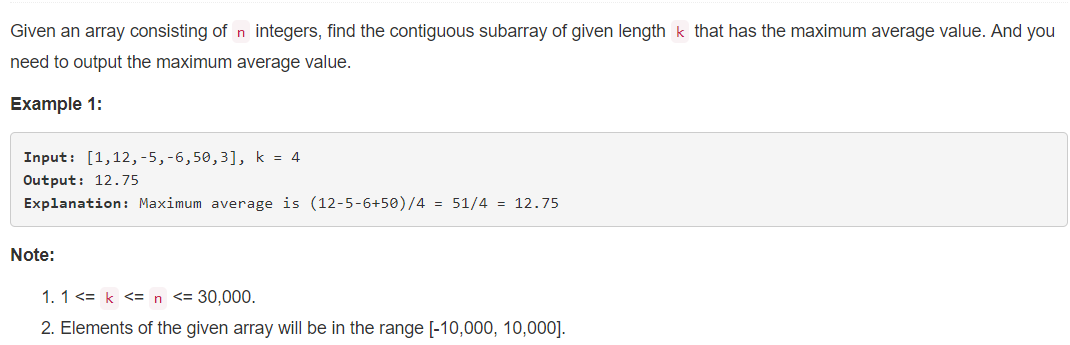
\includegraphics[width=18cm]{643.png}
	\end{center}
\end{figure}
\textbf{\large{Note:}}
\par
\vspace{0.5em}
This is a very easy problem.
\begin{itemize}
\item Get the sum of first $k$ numbers.
\item Starting from \texttt{index} $i = k$, subtract $nums[i - k]$ from and add $nums[i]$ into current sum.
\item Record maximum sum for each iteration.
\item Finally return the maximum sum divided by $k$.
\end{itemize}
\setcounter{algorithm}{0}
\begin{algorithm}[H]
\caption{Get maximum average for $k$ consecutive numbers}
\begin{algorithmic}
\Statex
\Procedure{Find-Max-Average}{$V$, $k$}
\State $sum := \sum\limits_{i=0}^{k-1}{V[i]} $ \Comment initially, get summation of first $k$ numbers
\For{$i \gets k, n-1$}
\State $sum := sum - V[i-k]$ \Comment remove first element of the sliding window $nums[i-k]$
\State $sum := sum + V[i]$ \Comment add current element $nums[i]$
\EndFor
\State \Return $sum \div k$
\EndProcedure
\Statex
\end{algorithmic}
\end{algorithm}

\subsection{644 -- Maximum Average Subarray II}
\begin{CJK*}{UTF8}{gbsn}
\begin{itemize}
\item 所求的最大平均值一定是介于原数组的最大值和最小值之间,所以用二分法来快速的在这个范围内找到要求的最大平均值。
\item 如果已经算出来了这个最大平均值,那么对于任意一个长度大于等于$k$的数组,如果让其中每个数字都减去这个平均值,那么得到的累加差值一定是小于等于$0$的。
\item 所以这个二分搜索开始前,左边界为数组最小值,右边界为数组最大值。
\item 每次判定下一次搜索范围时,看当前的中间值是否使得数组中存在某个连续部分中每个数与该值的差的和大于等于$0$。如果$\geq 0$,则这个值小了,左边界设定为\texttt{mid},否则右边界设定为\texttt{mid}。因为这个平均值不一定是整数,所以左右边界都要设置在\texttt{mid}。
\item 判定数组中是否存在某个连续部分中每个数与该值的差的和大于等于$0$,需要计算出从起始开始的连续数组和,然后同时看当前位置$k$位置之前的连续数组和的最小值,因为我们只需要判定是否有符合条件的存在。至于有多少个,不需要关心。
\end{itemize}
\clearpage
\end{CJK*}
\setcounter{algorithm}{0}
\begin{algorithm}[H]
\caption{Check if there exists a consecutive part  in which the summation of difference between each number and the given value is $\geq 0$}
\label{BinCheck}
\begin{algorithmic}
\Statex
\Procedure{Check}{$V$, $k$, $mid$}
\State $sum_{i} := 0$ \Comment prefix difference sum until \texttt{index} $i$
\State $sum_{i-k} := 0$ \Comment prefix difference sum until \texttt{index} $i-k$
\State $min_{sum}$ \Comment minimum prefix difference sum until \texttt{index} $i-k$
\For {$i \gets 0, k-1$}
\State $sum_{i}\gets sum_{i} + V[i] - \mathtt{mid} $
\EndFor
\If {$sum_{i} \geq 0$} \Comment The part is found
\State \Return \textbf{true}
\EndIf
\For {$i \gets k, L-1$} \Comment $L$ is the length of the array
\State $sum_{i}\gets sum_{i} + V[i] - \mathtt{mid}$
\State $sum_{i-k} \gets sum_{i-k} + V[i-k] - \mathtt{mid}$
\State update $min_{sum}$ as the minimum of $sum_{i-k}$ until now
\If {$min_{\mathtt{sum}} \leq sum_{i}$}  \Comment there is at least a consecutive part meet the condition
\State \Return \textbf{true}
\EndIf
\EndFor
\State \Return \textbf{false} \Comment there is no any consecutive part meet the condition
\EndProcedure
\Statex
\end{algorithmic}
\end{algorithm}

\begin{algorithm}[H]
\caption{Find the contiguous subarray whose length is greater than or equal to $k$ that has the maximum average value}
\begin{algorithmic}
\Statex
\Procedure{Find-Max-Avg}{$V$, $k$}
\State $\mathtt{left} := \min{V}$ \Comment get minimum element of the array
\State $\mathtt{right} := \max{V}$ \Comment get maximum element of the array
\While {$\mathtt{left} - \mathtt{right} \geq 10^{-6}$ } \Comment $10^{-6}$ is the minimum precision given in the question
\State $\mathtt{mid} := (\mathtt{left} + \mathtt{right})/2$ \Comment get the middle value.
\If{\textbf{Check}$(V,k,mid)$\ref{BinCheck} $=$ \textbf{true}}
\State $\mathtt{left} \gets mid$  \Comment \texttt{mid} is smaller, need to search in the right half
\Else
\State $\mathtt{right} \gets mid$ \Comment \texttt{mid} is greater, need to search in the left half
\EndIf
\EndWhile
\EndProcedure
\Statex
\end{algorithmic}
\end{algorithm}
\end{document}